	\section{Software-Entwicklung, Wartung und (Re)Engineering}
	Erstellte Software muss oft geändert werden, entweder aufgrund von geänderten Anforderungen oder neuen Anforderungen, welche eingebaut werden müssen.
	\subsection{Einleitung}
	\subsubsection{Geschichte}
	\begin{itemize}
		\item Softwarekrise 1968
		\item Nato \textbf{Working Conference on Software Engineering}
		\item Zuordnungen
		\begin{itemize}
			\item Praktische Informatik
			\item Theoretische Informatik
			\item Projektplanung
			\item Organisation
			\item Psychologie
			\item ...
		\end{itemize}
	\end{itemize}
	\subsubsection{''Software-Technik'' Definition}
	Software-Engineering(Software-Technik) ist nach \textbf{Entwicklung}, \textbf{Pflege} und \textbf{Einsatz}.
	\par 
	Eingesetzt werden:
	\begin{itemize}
		\item Wissenschaftliche Methoden
		\item Wirtschaftliche Prinzipien
		\item Geplante Vorgehensmodellen
		\item Werkzeuge
		\item Quantifizierbare Ziele
	\end{itemize}
	\subsubsection{50 Jahre nach Beginn der "Software-Krise"}
	\begin{itemize}
		\item 19\% aller Projekte sind gescheitert, früher 25\%
		\item 52\% aller Projekte sind dabei zu scheitern, früher 50\%
		\item 29\% aller betrachteten IT-Projekte sind erfolgreich, früher 25\%
	\end{itemize}
	Hauptgründe fürs Scheitern der Projekte:
	\par 
	Unklare Anforderungen und Abhängigkeiten sowie Problemen beim Änderungsmanagement.
	\subsection{Software-Qualität}
	Ziel der Software-Technik ist die effiziente Entwicklung messbar qualitativ hochwertiger Software.
	\par 
	\subsubsection{Qualitätsdefinition}
	Qualität ist der Grad, in dem ein System, eine Komponente oder ein Prozess die Kundenerwartungen und Kundenbedürfnisse erfüllt. 
	\subsubsection{Softwarequalität}
	Softwarequalität ist die Gesamtheit der Funktionalitäten und Merkmale eines Softwareprodukts, die sich auf dessen Eignung beziehen, festgelegte oder vorausgesetzte Erfordernisse zu erfüllen.
	\subsubsection{Qualitätsmerkmale}
	\begin{itemize}
		\item Funktionalität
	\end{itemize}
	\subsubsection{Nichtfunktionale Merkmale}
	\begin{itemize}
		\item Zuverlässigkeit (Reliability)
		\item Benutzbarkeit (Usability)
		\item Effizienz (Efficiency)
		\item Änderbarkeit (Maintainability)
		\item Übertragbarkeit (Portability)
	\end{itemize}
	\subsubsection{Prinzipien der Qualitätssicherung}
	\begin{itemize}
		\item \textbf{Qualitätszielbestimmung}: Auftraggeber und Auftragnehmer legen vor Beginn der Software-Entwicklung gemeinsames Qualitätsziel für Software-System mit nachprüfbaren Kriterienkatalog fest (als Bestandteil des abgeschlossenen Vertrags zur Software-Entwicklung)
		\item \textbf{Quantitative Qualitätssicherung}: Einsatz automatisch ermittelbaren Metriken zur Qualitätsbestimmung (objektivbare, ingenieursmäßige Vorgehensweise)
		\item \textbf{Konstruktive Qualitätssicherung}: Verwendung geeigneter Methoden, Sprachen und Werkzeuge (Vermeidung von Qualitätsproblemen)
		\item \textbf{Integrierte, frühzeitige, analytische Qualitätssicherung}: Systematische Prüfung aller erzeugter Dokumente (Aufdeckung von Qualitätsproblemen)
		\item \textbf{Unabhängige Qualitätssicherung}: Entwicklungsprodukte werden durch eigenständige Qualitätssicherungsabteilung überprüft und abgenommen (verhindert u.a. Verzicht auf Testen zugunsten Einhaltung des Entwicklungsplans)
	\end{itemize}
	\subsubsection{Konstruktives Qualitätssicherung zur Fehlervermeidung}: 
	\begin{itemize}
		\item Technische Maßnahmen
		\begin{itemize}
			\item Sprachen (UML, Java)
			\item Werkzeuge (UML-CASE-TOOL)
		\end{itemize}
		\item Organisatorische Maßnahmen
		\begin{itemize}
			\item Richtlinien (Gliederungsschema für Pflichtenheft, Programmierrichtlinien)
			\item Standards (für verwendete Sprachen, Dokumentformate, Management)
			\item Checklisten
		\end{itemize}
	\end{itemize}
	\subsubsection{Analytisches Qualitätsmanagement für Fehleridentifikation}
	\begin{itemize}
		\item \textbf{Analysierende Verfahren}: Der "Prüfling" (Programm, Modell, Dokumentation) wird von Menschen oder Werkzeugen auf Vorhandensein/Abwesenheit von Eigenschaften untersucht
		\begin{itemize}
			\item \textbf{Review}: Prüfung durch Menschen
			\item \textbf{Statische Analyse}: Werkzeuggestützte Ermittlung von "Anomalien"
			\item \textbf{Formale Verifikation}: Werkzeuggestützter Beweis von Eigenschaften
		\end{itemize}
		\item \textbf{Testende Vefahren}: Der "Prüfling" wird mit konkreten oder abstrakten Eingabewerten auf einem Rechner ausgeführt
		\begin{itemize}
			\item \textbf{Dynamischer Test}: "normale" Ausführung mit ganz konkreten Eingaben
			\item \textbf{Symbolischer Test}: Ausführung mit symbolischen Eingaben
		\end{itemize}
	\end{itemize}
	\subsection{Iterative Softwareentwicklung}
	Voraussetzung für den sinnvollen Einsatz von Notationen und Werkzeugen zur Software-Entwicklung ist ein:
	\begin{itemize}
		\item \textbf{Vorgehensmodell}, das den Gesamtprozess der Software-Erstellung und pflege in einzelne Schritte aufteilt
		\item Zusätzlich müssen Verantwortlichkeiten der beteiligten Personen in Form von \textbf{Rollen} im Software-Entwicklungsprozess klar geregelt sein.
	\end{itemize}
	\subsubsection{Übersicht der Phasen des Wasserfallmodells}
	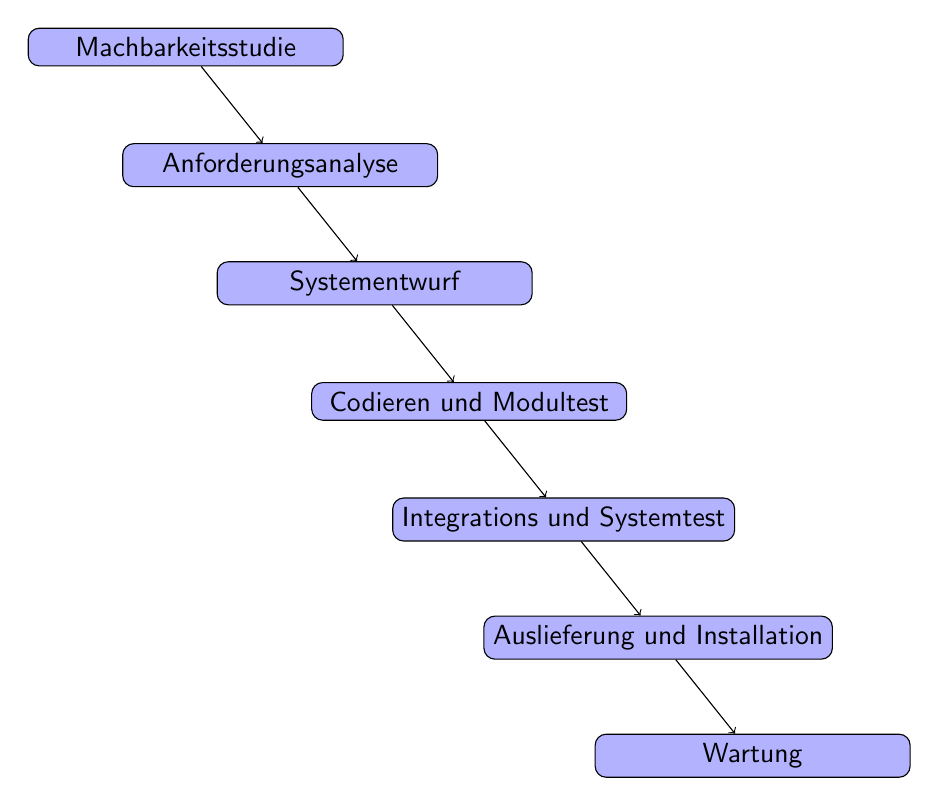
\begin{tikzpicture}[
		base/.style = {rectangle, rounded corners, draw=black,
		text centered, font=\sffamily},
		minimum width=4cm,
		blueStyle/.style = {base, fill=blue!30},]
		\node (machbarkeitsstudie) [blueStyle] {Machbarkeitsstudie};
		\node (anforderungsanalyse) [blueStyle, below of=machbarkeitsstudie, yshift=-0.5cm, xshift=1.2cm] {Anforderungsanalyse};
		\node (systementwurf) [blueStyle, below of=anforderungsanalyse, yshift=-0.5cm, xshift=1.2cm] {Systementwurf};
		\node (codieren) [blueStyle, below of=systementwurf, yshift=-0.5cm, xshift=1.2cm] {Codieren und Modultest};
		\node (integration) [blueStyle, below of=codieren, yshift=-0.5cm, xshift=1.2cm] {Integrations und Systemtest};
		\node (auslieferung) [blueStyle, below of=integration, yshift=-0.5cm, xshift=1.2cm] {Auslieferung und Installation};
		\node (wartung) [blueStyle, below of=auslieferung, yshift=-0.5cm, xshift=1.2cm] {Wartung};
		\draw[->] (machbarkeitsstudie) -- (anforderungsanalyse);
		\draw[->] (anforderungsanalyse) -- (systementwurf);
		\draw[->] (systementwurf) -- (codieren);
		\draw[->] (codieren) -- (integration);
		\draw[->] (integration) -- (auslieferung);
		\draw[->] (auslieferung) -- (wartung);
	\end{tikzpicture}
	\subsubsection{Machbarkeitsstudie (feasability study)}
	Die Machbarkeitsstudie schätzt Kosten und Ertrag der geplanten Software-Entwicklung ab. Dazu grobe Analyse des Problems mit Lösungsvorschlägen.
	\begin{itemize}
		\item \textbf{Aufgaben}
		\begin{itemize}
			\item Problem informell und abstrahiert beschreiben
			\item Verschiedene Lösungsansätze erarbeiten
			\item Kostenschätzung durchführen
			\item Angebotserstellung
		\end{itemize}
		\item \textbf{Ergebnisse}
		\begin{itemize}
			\item Lastenheft
			\item Projektkalkulation
			\item Projektplan
			\item Angebot an Auftraggeber
		\end{itemize}
	\end{itemize}
	\subsubsection{Anforderungsanalyse (requirements engineering)}
	In der Anforderungsanalyse wird exakt festgelegt, was die Software leisten soll, aber nicht wie diese Leistungsmerkmale erreicht werden.
	\begin{itemize}
		\item \textbf{Aufgaben}
		\begin{itemize}
			\item genaue Festlegung der Systemeigenschaften wie Funktionalität, Leistung, Benutzungsschnittstelle, Portierbarkeit, … im Pflichtenheft
			\item Bestimmen von Testfällen
			\item Festlegung erforderlicher Dokumentationsdokumente
		\end{itemize}
		\item \textbf{Ergebnisse}
		\begin{itemize}
			\item Pflichtenheft = Anforderungsanalysedokument 
			\item Akzeptanztestplan
			\item Benutzungshandbuch (1-te Version)
		\end{itemize}
	\end{itemize}
	\subsubsection{Systementwurf (system design/programming-in-the-large)}
	Im Systementwurf wird exakt festgelegt, wie die Funktionen der Software zu realisieren sind. Es wird der Bauplan der Software, die Software-Architektur, entwickelt.
	\begin{itemize}
		\item \textbf{Aufgaben}
		\begin{itemize}
			\item Programmieren-im-Großen = Entwicklung eines Bauplans
			\item Grobentwurf, der System in Teilsysteme/Module zerlegt
			\item Auswahl bereits existierender Software-Bibliotheken, Rahmenwerke, …
			\item Feinentwurf, der Modulschnittstellen und Algorithmen vorgibt
		\end{itemize}
		\item \textbf{Ergebnisse}
		\begin{itemize}
			\item Entwurfsdokument mit Software-Bauplan
			\item detaillierte(re) Testpläne
		\end{itemize}
	\end{itemize}
	\subsubsection{Codieren und Modultest (programming-in-the-small)}
	Die eigentliche Implementierungs- und Testphase, in der einzelne Module (in einer bestimmten Reihenfolge) realisiert und validiert werden.
	\begin{itemize}
		\item \textbf{Aufgaben}
		\begin{itemize}
			\item Programmieren-im-Kleinen = Implementierung einzelner Module
			\item Einhaltung von Programmierrichtlinien
			\item Code-Inspektionen kritischer Modulteile (Walkthroughs)
			\item Test der erstellten Module
		\end{itemize}
		\item \textbf{Ergebnisse}
		\begin{itemize}
			\item Menge realisierter Module
			\item Implementierungsberichte (Abweichungen vom Entwurf, Zeitplan, … )
			\item Technische Dokumentation einzelner Module
			\item Testprotokolle
		\end{itemize}
	\end{itemize}
	\subsubsection{Integrations- und Systemtest}
	Die einzelnen Module werden schrittweise zum Gesamtsystem zusammengebaut. Diese Phase kann mit der vorigen Phase verschmolzen werden, falls der Test isolierter Module nicht praktikabel ist.
	\begin{itemize}
		\item \textbf{Aufgaben}
		\begin{itemize}
			\item Systemintegration = Zusammenbau der Module
			\item Gesamtsystemtest in Entwicklungsorganisation durch Kunden (alpha-Test)
			\item Fertigstellung der Dokumentation
		\end{itemize}
		\item \textbf{Ergebnisse}
		\begin{itemize}
			\item Fertiges System
			\item Benutzerhandbuch
			\item Technische Dokumentation
			\item Testprotokolle
		\end{itemize}
	\end{itemize}
	\subsubsection{Auslieferung und Installation}
	Die Auslieferung (Installation) und Inbetriebnahme der Software beim Kunden findet häufig in zwei Phasen statt.
	\begin{itemize}
		\item \textbf{Aufgaben}
		\begin{itemize}
			\item Auslieferung an ausgewählte (Pilot-)Benutzer (Beta-Test)
			\item Auslieferung an alle Benutzer
			\item Schulung der Benutzer
		\end{itemize}
		\item \textbf{Ergebnisse}
		\begin{itemize}
			\item Fertiges System
			\item Akzeptanztestdokument
		\end{itemize}
	\end{itemize}
	\subsubsection{Wartung (Maintenance)}
	Nach der ersten Auslieferung der Software an die Kunden beginnt das Elend der Software-Wartung, das ca. 60\% der gesamten Software-Kosten ausmacht.
	\begin{itemize}
		\item \textbf{Aufgaben}
		\begin{itemize}
			\item ca. 20\% Fehler beheben (corrective maintenance)
			\item ca. 20\% Anpassungen durchführen (adaptive maintenance)
			\item ca. 50\% Verbesserungen vornehmen (perfective maintenance)
		\end{itemize}
		\item \textbf{Ergebnisse}
		\begin{itemize}
			\item Software-Problemberichte (bug reports)
			\item Software-Änderungsvorschläge
			\item Neue Software-Versionen
		\end{itemize}
	\end{itemize}
	\subsubsection{Probleme mit dem Wasserfallmodell}
	\begin{itemize}
		\item zu Projektbeginn sind nur ungenaue Kosten- und Ressourcenschätzungen möglich
		\item ein Pflichtenheft kann nie den Umgang mit dem fertigen System ersetzen, das erste sehr spät entsteht (Risikomaximierung)
		\item es gibt Fälle, in denen zu Projektbeginn kein vollständiges Pflichtenheft erstellt werden kann (weil Anforderungen nicht klar)
		\item Anforderungen werden früh eingefroren, notwendiger Wandel (aufgrund organisatorischer, politischer, technischer, … Änderungen) nicht eingeplant
		\item strikte Phaseneinteilung ist unrealistisch (Rückgriffe sind notwendig)
		\item Wartung mit ca. 60\% des Gesamtaufwandes ist eine Phase
	\end{itemize}
	\begin{figure}[h]
		\centering
		\caption{Andere Darstellung der Aufwandsverteilung}
		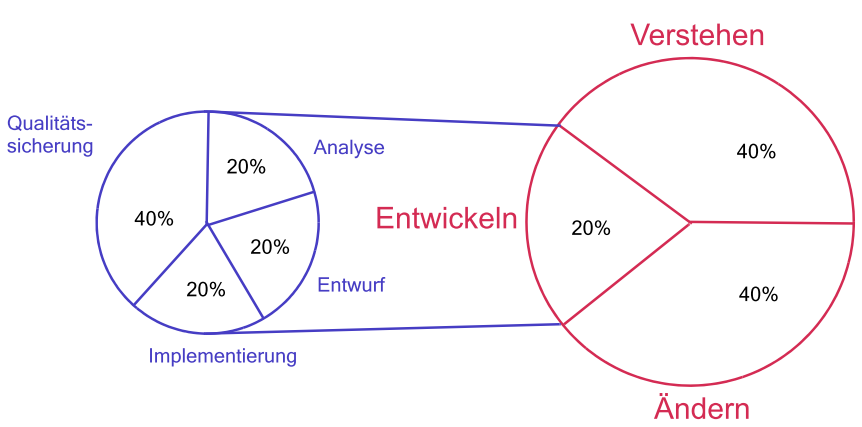
\includegraphics[width=0.65\textwidth]{taskDistribution}
	\end{figure}
	\subsubsection{Typische Probleme in der Wartungsphase}
	\begin{itemize}
		\item Einsatz wenig erfahrenen Personals (nicht Entwicklungspersonal)
		\item Fehlerbehebung führt neue Fehler ein
		\item Stetige Verschlechterung der Programmstruktur
		\item Zusammenhang zwischen Programm und Dokumentation geht verloren
		\item Zur Entwicklung eingesetzte Werkzeuge (CASE-Tools, Compiler, … ) sterben aus
		\item Benötigte Hardware steht nicht mehr zur Verfügung
		\item Resourcenkonflikte zwischen Fehlerbehebung und Anpassung/Erweiterung
		\item Völlig neue Ansprüche an Funktionalität und Benutzeroberfläche
	\end{itemize}
	\subsection{Forward-, Reverse- und Reengineering}
	\subsubsection{Software Evolution}
	\begin{itemize}
		\item Wünsche
		\begin{itemize}
			\item Wartung ändert Software kontrolliert ohne Design zu zerstören
			\item Konsistenz aller Dokumente bleibt erhalten
		\end{itemize}
		\item Wirklichkeit
		\begin{itemize}
			\item Ursprüngliche Systemstruktur wird ignoriert
			\item Dokumentation wird unvollständig oder unbrauchbar
			\item Mitarbeiter verlassen Projekt
		\end{itemize}
	\end{itemize}
	\subsubsection{Forward Engineering}
	Beim Forward Engineering ist das fertige Softwaresystem das Ergebnis des Entwicklungsprozesses. Ausgehend von Anforderungsanalyse (Machbarkeitsstudie) wird ein neues Softwaresystem entwickelt.
	\subsubsection{Reverse Engineering}
	Beim Reverse Engineering ist das vorhandene Software-System der Ausgangspunkt der Analyse. Ausgehend von existierender Implementierung wird meist „nur“ das Design rekonstruiert und dokumentiert. Es wird (noch) nicht das betrachtete System modifiziert.
	\subsubsection{Reengineering}
	Reengineering befaßt sich mit der Sanierung eines vorhandenen Software-Systems bzw. seiner Neuimplementierung. Dabei werden die Ergebnisse des Reverse Engineerings als Ausgangspunkt genommen
	\begin{figure}[h]
		\centering
		\caption{Round Trip Engineering}
		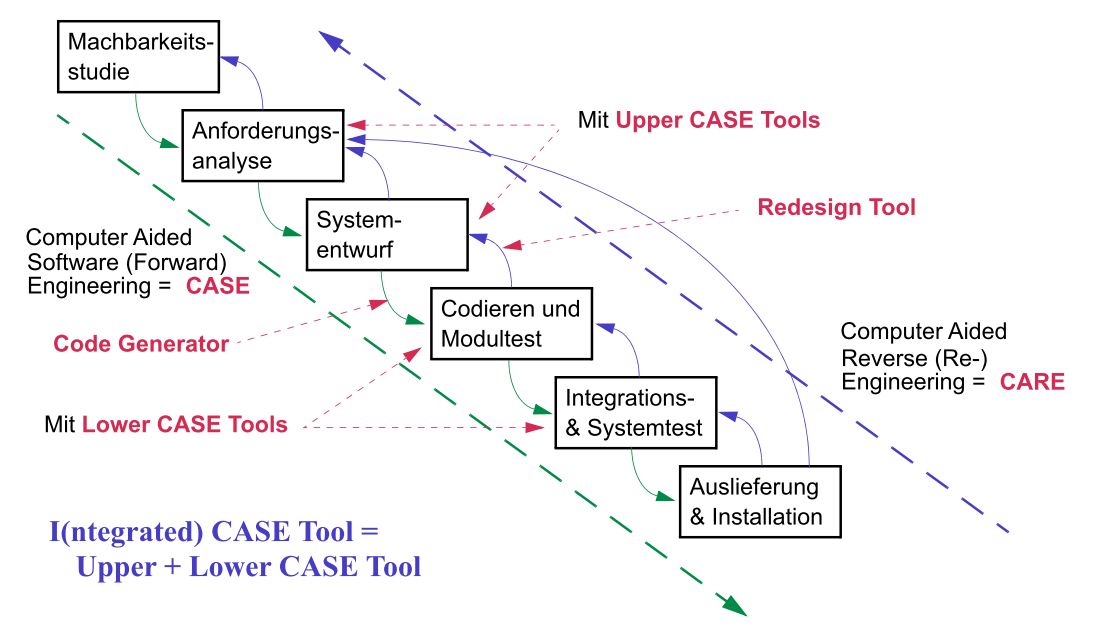
\includegraphics[width=0.85\textwidth]{roundTripEngineering}
	\end{figure}
	\begin{figure}[h]
		\centering
		\caption{Einfaches Software-Lebenszyklus-Prozessmodell für die Wartung}
		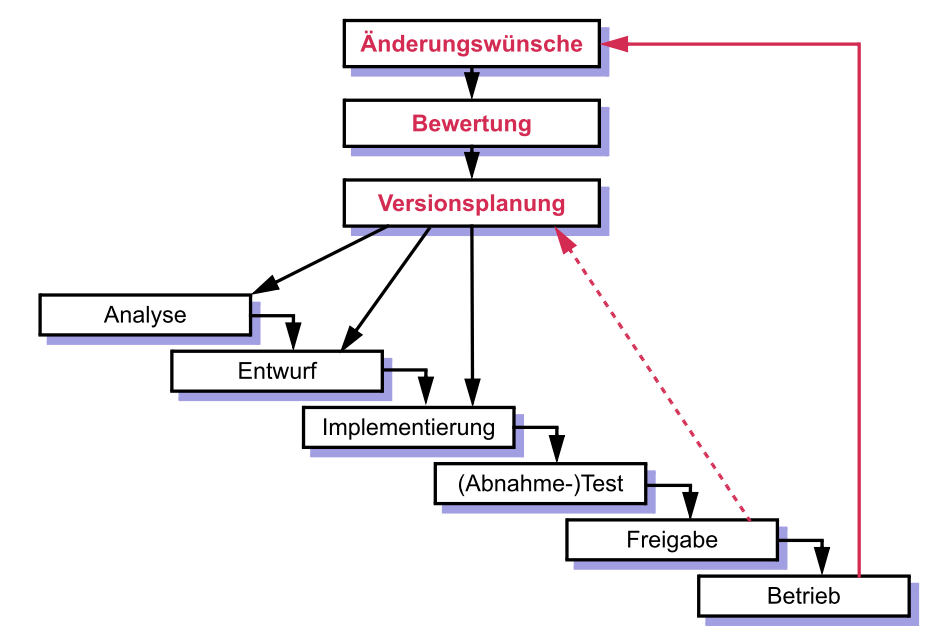
\includegraphics[width=0.85\textwidth]{softwareCycle-1}
	\end{figure}
	\subsubsection{Das V-Modell}
	\begin{itemize}
		\item \textbf{Systemanforderungsanalyse}: Gesamtsystem einschließlich aller Nicht-DV-Komponenten wird beschrieben (fachliche Anforderungen und Risikoanalyse)
		\item \textbf{Systementwurf}: System wird in technische Komponenten (Subsysteme) zerlegt, also die Grobarchitektur des Systems definiert
		\item \textbf{Softwareanforderungsanalyse}: Technischen Anforderungen an die bereits identifizierten Komponenten werden definiert
		\item \textbf{Softwaregrobentwurf}: Softwarearchitektur wird bis auf Modulebene festgelegt
		\item \textbf{Softwarefeinentwurf}: Details einzelner Module werden festgelegt
		\item \textbf{Softwareimplementierung}: Wie beim Wasserfallmodell (inklusive Modultest) 
		\item \textbf{Software-/Systemintegration:}: Schrittweise Integration und Test der verschiedenen Systemanteile
		\item \textbf{Überleitung in die Nutzung:}: Entspricht Auslieferung bei Wasserfallmodell
	\end{itemize}
	\begin{figure}[h]
		\centering
		\caption{Das V-Modell}
		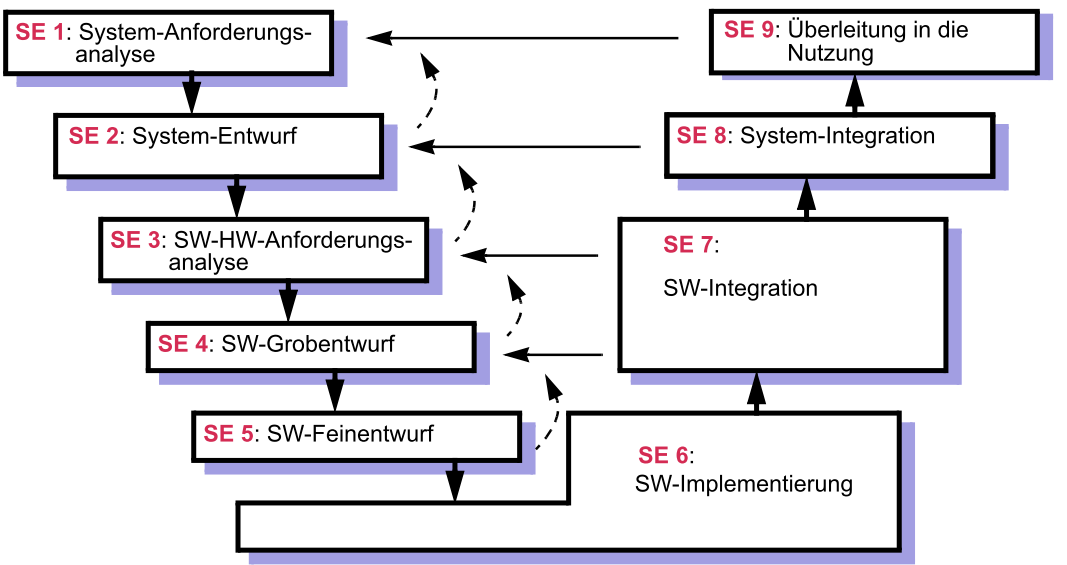
\includegraphics[width=0.85\textwidth]{v-model}
	\end{figure}
